% !TeX spellcheck = en_US
\documentclass{article}
\usepackage[utf8]{inputenc}
\usepackage[T1]{fontenc} 
\usepackage[english]{babel}

\usepackage{amsmath}
\usepackage{amsthm}
\usepackage{amssymb}
\usepackage{amsfonts}
\usepackage{mathtools}
\usepackage{newtxtext}
\usepackage{newtxmath}

\usepackage{microtype}
\usepackage{floatflt}

\usepackage{graphicx}

\usepackage{hyperref}
\usepackage[backend=bibtex]{biblatex} %I need to use biblatex for some special features

\usepackage{mdframed}
\mdfsetup{skipabove=\topskip,skipbelow=\topskip}
\global\mdfdefinestyle{exampledefault}{%
outerlinewidth=5pt,innerlinewidth=0pt,outerlinecolor=red,roundcorner=5pt
}

% ------------- Geometry ---------------------------
\usepackage{geometry}
\geometry{
	a4paper,
	total={170mm,257mm},
	left=25mm,
	right=25mm,
	top=20mm,
}
% ------------- MATHEMATICAL ENVIRONMENTS ----------
\newcommand{\R}{\mathbb{R}}
\newcommand{\C}{\mathbb{C}}
\newcommand{\tu}{\tilde{U}}
\renewcommand{\hat}{\widehat}
\renewcommand{\phi}{\varphi}
\newcommand{\diff}{\mathop{}\!d}
\newcommand{\norm}[1]{\left\lvert #1\right\rvert}
\newcommand{\pd}[2]{\frac{\partial #1}{\partial #2}}
\newcommand{\pds}[2]{\frac{\partial^2 #1}{\partial #2^2}}

% ------------- IMPORTARE CODICE IN MATLAB/OCTAVE --
\usepackage{listings}
\usepackage{color}
\usepackage{bigfoot} % to allow verbatim in footnote
\usepackage[numbered,framed]{matlab-prettifier}

\usepackage{filecontents}

\let\ph\mlplaceholder % shorter macro
\lstMakeShortInline"

\lstset{
	style              = Matlab-editor,
	basicstyle         = \mlttfamily,
	escapechar         = ",
	mlshowsectionrules = true,
}

\usepackage{titling}

\pretitle{%
	\begin{center}
		\LARGE
		
\includegraphics[height=2cm]{image}\\[\bigskipamount]
	}
\posttitle{\end{center}}



% ---------------- BIGIN OF THE WORK -----------------
\begin{document}
\date{\today}
\author{Neil Abhra Chowdhury \& Enrique Sanchez del Villar, Erik Pillon}
\title{Finite Elements Project}
\maketitle
\begin{abstract}
	This is the final project of the course \textbf{Numerical Methods}, given at Phelma in the Academic Year 2017/2018. In this project we will study a process of material elaboration involving heating by electrode. We 'll study the steady state of this process. The objective is to model the physical phenomena which take place in this process with \emph{finite element method}.
	
	All the source code, matlab \textit{m files} and figures can be found on the Github repository \url{https://github.com/ErikPillon/NumericalMethods}
\end{abstract}

\section{Statement of the Problem}
The study configuration is considered cylindrical. A scheme of the study geometry is given in Figure~\ref{figure:problem}:
\begin{figure}
	\centering
	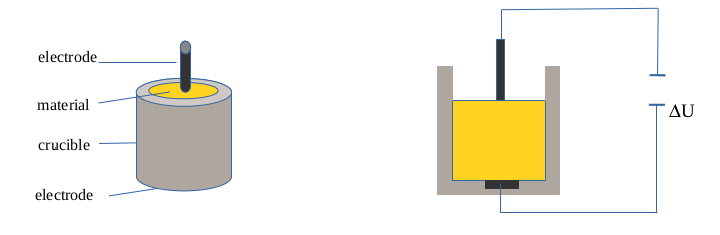
\includegraphics[height=4cm]{Images/problem.png}
	\caption{Problem Scheme}
	\label{figure:problem}
\end{figure}
The process is constituted by:
\begin{itemize}
	\item a cylindrical crucible;
	\item the elaborated material; the geometry of the study domain occupied by the material is cylindrical;
	\item 2 electrodes.
\end{itemize}

The electrodes are in graphite. An electrical potential difference is applied between the top electrode and the bottom electrode included in the crucible: $ \Delta U $. This electrical potential difference is \emph{continuous}. An electrical current pass through the material placed in the crucible. We suppose that the contact between the electrodes and elaborated material is perfect. \textbf{Joule effect heat the material}. The material of the crucible is an insulating material. The crucible is not model and will be replaced by an adapted boundary condition. Electrical problem has to be solved in the electrodes and in the elaborated material. The heat transfer has to be solved in the material only.

\section{Equations of the physical phenomenon and Boundary Conditions}
The objective of this part is to present the physical equations of the process in the steady state and boundary conditions. In this process two physical phenomena occur:
\begin{itemize}
	\item electrical phenomenon;
	\item thermal phenomenon.
\end{itemize}
\subsection{Presentation of the study domain}
Describe the study domain. Precise where each phenomenon is solved.
\begin{mdframed}
	The study domain is the one described in Figure~\ref{figure:problem}, right part. 
	\begin{itemize}
		\item We will solve the \textbf{thermal problem} only in the material only (yellow part), i.e.~where $ 0.1<r<0.3 $ and $ 0<h<0.3 $.
		\item We will solve the \textbf{electrical problem} in the electrodes and in the elaborated material, i.e.~for $ 0\geq r<0.3 $ and $ 0<h<0.3 $.  
	\end{itemize} 
\end{mdframed}
\subsection{Electrical problem}
Give the partial differential equation of the electrical problem.
Give the boundary conditions of the electrical problem.
Give the expression of the current density and of the Joule power density.
\begin{mdframed}
	The Electrical problem can be modeled employing the fact that $ E=-\nabla U $. We also now that the electrical flux is defined through $ \vec{J}\cdot \vec{E} $. Using the fact that the divergence of the Electrical flux is 0 we obtain that:
	\[ \nabla\cdot(-\sigma\nabla U)=0. \]
	We focus now on the boundary conditions: we know that around the crucible there's insulator material, then we'll have that $ \pd{U}{x}=0 $ on the boundary, i.e. $ \nabla U\cdot \vec{n}=0 $. We can also take into consideration that $ \Delta U $ is fixed and so we can write the final system as
	\[
	\begin{cases}
	\nabla\cdot(-\sigma\nabla U)=0, & 0<x<0.1,\,0.02<z<0.42\\
	\nabla U\cdot \vec{n}=0,& x\in \partial V\\
	U = \Delta U, & 0<x<0.02,\,z=0.4\\
	U=0, & 0<x<0.04,\,z=0.
	\end{cases}
	\]
\end{mdframed}

\subsection{Thermal problem}
\begin{itemize}
	\item Give the partial differential equation of the thermal problem.
	\item Give the boundary conditions of the thermal problem.
\end{itemize}
\begin{mdframed}
	The Fourier Law tells us that:
	\begin{equation}
	\label{eq:Fourier}
	q=-k\nabla T
	\end{equation}
	where
	\begin{description}
		\item[$ q$] local heat flux density,
		\item[$ k $] material's conductivity,
		\item[$ \nabla T $] is the temperature gradient. 
	\end{description}
	From the Gauss-Green theorem we know that 
	\[
	\iint_S q(x,y,z) \diff S=Q
	\]
	where the first integral is all over the surface defined by $ 0.1<r<0.3 $ and $ 0<h<0.3 $ and $ Q $ is the heat generated by the Joule effect.
	
	By the way, employing the divergence theorem, the left hand side of the equation can be rewritten as  
	\[ \iiint \nabla\cdot q(x,y,z) \diff x\diff y\diff z = \iint_S q(x,y,z) \diff S  \]
	and then the following identity holds
	\begin{equation}
	\iiint \nabla\cdot q(x,y,z) \diff x\diff y\diff z = Q.
	\end{equation}
	Using Fourier Law \eqref{eq:Fourier} and plugging it into the above equation we obtain
	\begin{equation}
	\nabla\cdot(-k\nabla T)=Q.
	\end{equation}
	The final system of equation will be
	\begin{equation}
	\label{problem:heat}
	\begin{cases}
		\nabla\cdot(-k\nabla T)=Q, \\
		-\kappa\nabla T\cdot \vec{n}=h(T-T_r)
	\end{cases}
	\end{equation}
\end{mdframed}

	
\section{Principle of the Modeling}
In this project, in a first step, each equation will be developed and test. In a second step, the model with the
two coupling equations will be developed and test. For numerical modeling the finite element method is
used. In this project, describe the steps of the calculation and the variables used. Take time to define how you
will present your numerical results.

% !TeX spellcheck = en_US
\section{Numerical Modeling of Heat Transfer Problem with Finite Elements Method}
\subsection{Study Domain and Mesh}
\label{sec:4.1}
\begin{figure}
	\centering
	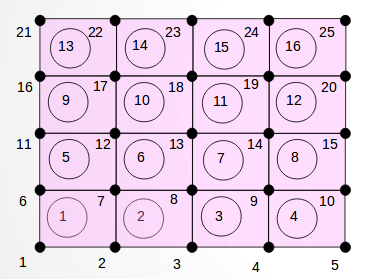
\includegraphics[height=4cm]{Images/mesh.png}
	\caption{Discretization of the domain.}
	\label{figure:mesh}
\end{figure}
\begin{mdframed}
	We want to discretize our domain in the same way described in figure \ref{figure:mesh}.
	
	The variable that we are going to use will be the \emph{length and the height of the domain}, as well as the \emph{number of the point} we want in our discretization. 
	
	A simple algorithm that takes care of that could be the one in Listing \ref{points}, where we have put in input of our function \texttt{mesh} the number of points in which we want to discretize our domain \texttt{nx,ny}.   
	
	\lstinputlisting[label={points},caption={Mesh}]{Matlab_Code/points.m}
	
	We stress the fact that in "for"~loop we take care also of the fact that if the point considered is a boundary point we have to come back and restart in \emph{another line}.
	
	The algorithm presented in Listing \ref{mesh} takes care of numbering in a proper way the elements basis and the points we have generated with the alorithm \texttt{points}.
	\lstinputlisting[label={mesh},caption={Build relationship for local point and overall point}]{Matlab_Code/mesh.m}
	
	In Listing \ref{b_points_electric} we give an algorithm for the mesh of the boundary elements.  
	\lstinputlisting[label={b_elements_electric},caption={Algorithm for boundary elements}]{Matlab_Code/b_elements.m}
\end{mdframed}
\subsection{Galerkin’s Formulation of Heat Transfer Equation}
\subsubsection{Projection of the partial differential equation on an element of the basis of the functions $ \alpha_i $}
We want to evaluate at this stage the projection of our unknown function $ T $ into the element basis $ \beta_i $, i.e., $ \forall i $ we want 
\begin{equation}
\label{eq:proj}
\iiint_{\Omega}\beta_i\nabla\cdot(-\kappa\nabla T)\diff\Omega=\iiint_{\Omega}\beta_i Q\diff\Omega
\end{equation} 
Now we can identify the element basis $ \beta_i $ with the element basis $ \alpha_i $ and so we can write  
\[\iiint_{\Omega}\alpha_i\nabla\cdot(-\kappa\nabla T)\diff\Omega=\iiint_{\Omega}\alpha_i Q\diff\Omega \]

\subsubsection{Give the weak formulation of the Galerkin’s method. Introduce the boundary conditions in the formulation.}
\begin{mdframed}
	Using the differential identity 
	\[\nabla\cdot(-\alpha_i)\kappa\nabla T)=-\alpha_i\nabla\cdot(\kappa\nabla T)-\kappa\nabla\alpha_i\nabla T\]
	we can plug the above equation into \eqref{eq:proj} obtaining 
	
	\[\iiint_{\Omega}\nabla\cdot(-\alpha_i)\kappa\nabla T\diff\Omega+\iiint_{\Omega}\kappa\nabla\alpha_i\nabla T\diff\Omega=\iiint_{\Omega}\alpha_i Q\diff\Omega\]
	
	By the way, we have, thanks to the divergnece theorem, that 
	\[\iiint_{\Omega}\nabla\cdot(-\alpha_i)\kappa\nabla T\diff\Omega=-\iint_{\Gamma}\alpha_i\kappa\nabla T\cdot\vec{n}\diff\Gamma. \]
	
	Then finally we have the \textbf{weak formulation of the problem} \eqref{eq:proj}
	\[ \iiint_{\Omega}\kappa\nabla\alpha_i\nabla T\diff\Omega-\iint_{\Gamma}\alpha_i\kappa\nabla T\cdot\vec{n}\diff\Gamma=\iiint_{\Omega}\alpha_i Q\diff\Omega. \]
	\medskip
	
	Introducing the boundary conditions, see \eqref{problem:heat}, we have
	\[\begin{cases}
	-\kappa\nabla T\cdot \vec{n}=h(T-T_r),& \text{on the free surface}\\
	-\kappa\nabla T\cdot \vec{n}=0,&\text{on all the non-free surface}\\
	\end{cases}\]
	and then 
	\begin{equation}
	\forall i \iint_{\Gamma}\alpha_i h(T-T_r)\diff\Gamma+\iiint_{\Omega}\kappa\nabla\alpha_i\nabla T\diff\Omega =\iiint_{\Omega}\alpha_i Q\diff\Omega
	\end{equation}
\end{mdframed}
\subsubsection{Precise the expression of the elementary volume, the elementary surface for respectively the volume integral and surface integral.}
\begin{mdframed}
	The idea is to transform an integral all over the volume $ \Omega $ in many sums all over the small elements $ e $. The elements must be disjoint pairwise and the union of the small elements $ e $ must be give the original volume $ \Omega $. In symbols we have
	\[\iiint_{\Omega}\left[\dots\right]\diff\Omega=\sum_e\iiint_{\omega_e}\left[\dots\right]\diff\Omega_e \]
	Similarly we'll have that the integral all over the susface is made up by the sum by the sum of all the small surfaces:
	\[\iint_{\Gamma}\left[\dots\right]\diff\Gamma=\sum_f\iint_{\gamma_f}\left[\dots\right]\diff\Gamma_f \] 
	
	We use the canonical change of variable, from cartesian to cylindrical, i.e., \begin{align}\label{change}
	(x,y,z)&\to(r,\theta,z)\\
	(x,y,z)&\mapsto(rcos(\theta),rsin(\theta),z)\nonumber
	\end{align}
	The change of variable given by Eq.\ref{change} gives as determinant of the Jacobian matrix the element $ r $, in such a way that the integration must be performed changing $ \diff x\diff y\diff z $ into $ r\diff r\diff\theta\diff z $.
	
	Then we have that 
	\[ 2\pi\iint_{\Omega}\kappa\nabla\alpha_i\nabla T\,r\diff r\diff z-2\pi\int_{\Gamma}\alpha_i\kappa\nabla T\cdot\vec{n}\diff z=2\pi\iint_{\Omega}\alpha_i Q\,r\diff r\diff z. \]
	
	In particular we will perform this transformation
	\[\iint_ef(x,y)\diff x\diff y=\int_{-1}^1\int_{-1}^1f(x(u,v),y(u,v))det(Jac)\diff u\diff v \]
	where \\
	\begin{minipage}{\linewidth}
		\begin{minipage}{.325\linewidth}
			\[\begin{cases}
			x(u,v)=\sum_{i=1}^{N}\alpha_i(u,v)\cdot x_i\\
			y(u,v)=\sum_{i=1}^{N}\alpha_i(u,v)\cdot y_i
			\end{cases}\]
		\end{minipage}
		and
		\begin{minipage}{.675\linewidth}
			\[
			\det(Jac)=\begin{vmatrix}
			\pd{x}{u}&\pd{y}{u}\\
			\pd{x}{v}&\pd{y}{v}
			\end{vmatrix}
			=
			\begin{vmatrix}
			\sum_{i=1}^{N}\frac{\partial\alpha_i(u,v)}{\partial u}\cdot x_i &\sum_{i=1}^{N}\frac{\partial\alpha_i(u,v)}{\partial u}\cdot y_i\\
			\sum_{i=1}^{N}\frac{\partial\alpha_i(u,v)}{\partial v}\cdot x_i &\sum_{i=1}^{N}\frac{\partial\alpha_i(u,v)}{\partial v}\cdot y_i
			\end{vmatrix}
			\]
		\end{minipage}
	\end{minipage}
	and therefore the integral we have to evaluate become a summation with a suitable quadrature formula
	\[\iint_ef(x,y)\diff x\diff y= \sum_{i\in\{nodes\}}f(x(u_i,y_i),y(u_i,y_i))\det(J(u_i,y_i))w_i \]
\end{mdframed}
\subsubsection{Give the expression of the integrals on the reference element}
The expression for each element of the basis is then
\[\sum_j \iiint_{e}\nabla\alpha_i\nabla\alpha_j\xi\diff\xi\diff\eta. \] 

Let's notice that we have 
\[T=\sum_{j=1}^N\alpha_j(\xi,\eta,\zeta)\cdot T_j \]
and so the differential becomes
\[\nabla T=\sum_{j=1}^N\nabla\alpha_j(\xi,\eta,\zeta)\cdot T_j \]
where through elementary calculations we can see that 
\[\nabla \alpha_j=\begin{bmatrix} Jac J \end{bmatrix}^{-1}\begin{bmatrix}
\pd{\alpha}{\xi}\\\pd{\alpha}{\eta}\\\pd{\alpha}{\zeta} 
\end{bmatrix}. \]

Then the final expression will be
\begin{align*}
\sum_e\iint_{\omega_e}\kappa\nabla\alpha_i\cdot\left(\sum_{j=1}^{N}\nabla\alpha_jT_j \right) \xi\diff\xi\diff\eta +\sum_f\int_{\Gamma}\alpha_ih\left(\sum_{j=1}^{N}\alpha_jT_j\right)\diff \eta=
\sum_f\int_{\Gamma}\alpha_ihT_r\diff \eta+\sum_e\iiint_{\omega_e}\alpha_iQ\,\xi\diff\xi\diff\eta.
\end{align*}


\subsubsection{Detail the expression of the elementary matrix on an element $ e $. Precise the size of each elementary matrix (sub matrix). Precise the expression of each integral and the principle of calculation. For each integral, precise the nature of the element $ e $} 

The elementary matrix of an element $ e $ is given by the inner product $ \nabla\alpha_i\nabla\alpha_j $. In particular we'll have a matrix $ A_{ij}^e $ in which we will have in position $ (i,j) $ the element $ \nabla\alpha_i\nabla\alpha_j $. 
The matrix will be evaluated through a 2-dimensional quadrature formula; in 1-dimension quadrature formula allow us to pass from a continuous integral to a discrete sum of values. First of all we have to rescale the integral extrema to 1 and -1,
\[\int_{a}^{b}f(x)\,dx = \frac{b-a}{2}\int_{-1}^{1}f\left(\frac {b-a}{2}x+ \frac{a+b}{2}\right)\, dx. \]
Then the discretization will become
\[ \frac{b-a}{2} \sum_{i=1}^{n}w_{i}f\left(\frac {b-a}{2}x_{i}+ \frac{a+b}{2}\right),\]
where suitable values $ x_i $ and weights $ w_i $ will be taken.

The matrix $ A_{ij}^e $ is a $ 4\times4 $ matrix, for each inner element. For the outer element it will be a $ 2\times2 $ matrix. 
\begin{figure}
	\centering
	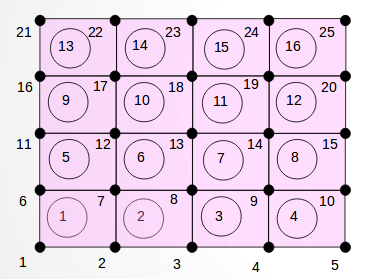
\includegraphics[height=4cm]{Images/mesh.png}
	\caption{The boundary elements will have 3 boundaries or 2, depending on which one we are considering.}
\end{figure}


% !TeX spellcheck = en_US
\subsection{Algorithm of the Finite Element Formulation of Heat Transfer Equation}
The algorithm goes as follows:
\begin{mdframed}
	\begin{itemize}
		\item Discretize the domain and build the mesh.
		\item Initialize the variables like heat conductivity, electrical conductivity, room Temperature, the Gauss nodes. 
		\item For each element $ e $ of the domain:
		\begin{itemize}
			\item Construct the Jacobian matrix $ Jac $ with the functions $ \alpha_i $
			\item Evaluate the Jacobian $ \det(Jac) $
			\item Evaluate all the 16 terms $ \nabla\alpha_i\nabla\alpha_j $ with the help of the Gauss quadrature formula.
			\item Update the global matrix $ A $ with the function \texttt{Update}
		\end{itemize}
		\item For each element $ f $ of the upper boundary:
		\begin{itemize}
			\item Construct the Jacobian $ Jac $ with the functions $ \alpha_1 $ and $ \alpha_2 $
			\item Evaluate all the 4 terms $ \alpha_i\alpha_j $ with the help of the 1D Gauss quadrature formula.
			\item Add the source term for the nearest neighbor.
			\item Update the global matrix $ B $ with the function \texttt{Update} modified for the boundary elements
		\end{itemize}
		\item Solve the linear problem $ (A_{ij}+B_{ij})T_i = \text{rhs} $
	\end{itemize}
	
\end{mdframed}


In the program we make use of the following functions:
\begin{itemize}
	\item \texttt{jacobian(M, Elem, e)} where \texttt{M} is the coordinates matrix and \texttt{Elem} is the mesh matrix, while \texttt{e} is the global element taken into consideration.
	\item \texttt{alpha(xi,eta)} where \texttt{xi,eta} are the local coordinates.
	\item \texttt{update} for updating the global matrix with the 16 values obtained for each element $ e $. 
	\item The functions \texttt{points} and \texttt{mesh} as already stated in Section \ref{sec:4.1} 
	\item \texttt{heat\_contribution}
	\item \texttt{integral\_1D}
	\item The function \texttt{Update} for putting the values of the local matrix of each element $ e $ (resp. $ f $) in the global matrix $ A $ (resp. $ B $).
	\item \texttt{Update\_rhs}
	\item \texttt{neumann\_condition} for evaluating the contribution given only on the upper free surface.
\end{itemize}


In Fig.~\ref{fig:non-coupled_thermal_problem} is plotted the 3D mesh of the non coupled solution for the Thermal Problem. 
\begin{figure}[htbp]
	\centering
	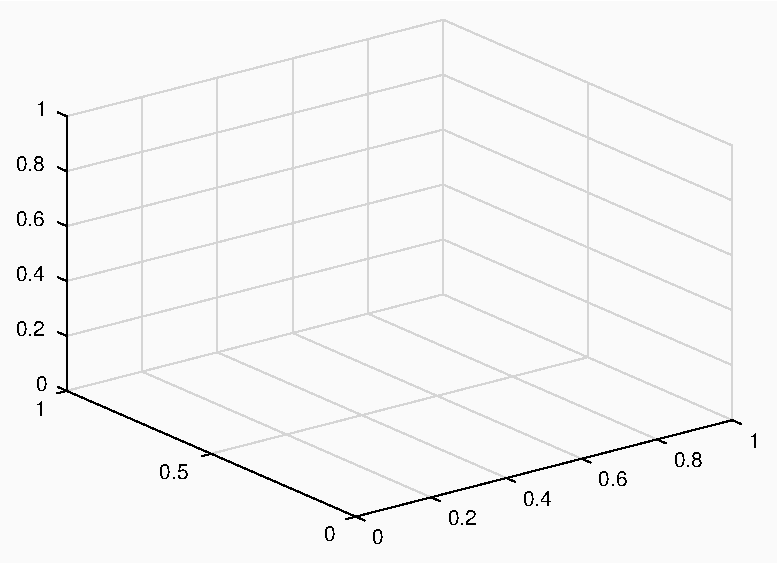
\includegraphics{Matlab_Code/Temperature_result}
	\caption{Result for the non-coupled thermal problem}
	\label{fig:non-coupled_thermal_problem}
\end{figure}



\subsection{Programming and calculation}
\subsubsection{Construct the program: main program and functions}
In the following we paste the code used in the resolution of the thermal problem. 
Listing \ref{main} is the \texttt{main} file used for the resolution. In the middle we've used several different functions, that are listed below.

\lstinputlisting[label={main},caption={main program},lastline=85]{Matlab_Code/main.m}

Where we used the function \texttt{jacobian}, \texttt{alpha}, \texttt{update} and \texttt{dIntegral} listed below.

\lstinputlisting[label={jacobian},caption={function for the creation of the jacobian matrix for each element}]{Matlab_Code/jacobian.m}


The function \ref{alpha} is used for the creation of the alpha functions $ \alpha_i $ which will be used as the element basis of the local elements.
\lstinputlisting[label={alpha},caption={Function for the creation of the alpha functions and the derivatives of the latter}]{Matlab_Code/alpha.m}

The function \ref{update_thermal} is used for updating the global matrix with the values evaluated for each element of the domain and properly put in position $ (i,j) $.
\lstinputlisting[label={update_thermal},caption={Function for update the global matrix with the values obtained for the local element $ e $}]{Matlab_Code/Update.m}

\lstinputlisting[label={dIntegral},caption={Function for evaluating the double integral$ \iint\nabla\alpha_i\nabla\alpha_j $}]{Matlab_Code/double_integral.m}

The function \ref{Updaterhs} is used for updating the right hand side of the equation with all the contributions evaluated for every boundary element.
\medskip

\lstinputlisting[label={Updaterhs}, caption={Update the right hand side of the equation}]{Matlab_Code/Update_rhs.m}

\lstinputlisting[caption={Function for evaluating the contribution given by the Joule effect. For the non coupled problem $ Q $ will be considered constant and equal to 1}]{Matlab_Code/heat_contribution.m}

\lstinputlisting[caption={Update the global matrix of the problem with the boundary conditions}]{Matlab_Code/Update_boundary.m}

The function \ref{neumann} is used for taking into account the neumann boundary conditions in the problem.
\lstinputlisting[label={neumann}, caption={neumann}]{Matlab_Code/neumann_condition.m}


% !TeX spellcheck = en_US
\section{Model the Electrical Problem with the Finite Elements Method}
\subsection{Study Domain and Mesh}

\begin{figure}[htbp]
	\begin{minipage}[c]{.5\linewidth}
		Since the domain of interest of the electric problem is larger than the thermal problem, we have to slightly modify our algorithm. We then have the algorithm in Listing \ref{points_electric}, where we have put in input of our function \texttt{mesh electric} the number of points in which we want to discretize our domain. In Fig.~ is painted the domanin of interest for this part of the problem.   
	\end{minipage} \hfill
	\begin{minipage}[c]{.5\linewidth}
		\centering
		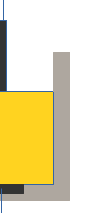
\includegraphics[height=3cm]{Images/electric_domain.png}
		\caption{Domain of interest of the electric part}
		\label{figure:electric_domain}
	\end{minipage}
\end{figure}

\lstinputlisting[label={points_electric},caption={Points}]{Matlab_Code/points_electric.m}


\lstinputlisting[label={mesh_electric},caption={Build relationship for local point and overall point}]{Matlab_Code/mesh_electric.m}

\subsection{Galerkin’s Formulation of the Electrical Equation}
The projection of the partial differential equation on a basis element is
\[\iiint_{\omega} \alpha_i \nabla\cdot(-\sigma\nabla U)\diff\Omega=0, \quad \forall i \]
and then the \textbf{weak formulation for the electric part} becomes
\begin{equation}
\iiint_{\omega}\sigma\alpha_i\cdot\nabla U\diff \Omega=0,\quad \forall i.
\end{equation}
The boundary conditions given can be modelized in the following fashion
\[\begin{cases}
U = 0, &\text{on the top of the crucible,}\\
U = U_0, &\text{on the bottom of the crucible,}\\
J\cdot n=0, &\text{on all the other surfaces.}
\end{cases} \]
As before, the elementary element of surface and volume are given by the canonical change of variables, from cartesian to cylindrical, i.e., \begin{align}\label{change2}
(x,y,z)&\to(r,\theta,z)\\
(x,y,z)&\mapsto(rcos(\theta),rsin(\theta),z)\nonumber
\end{align}
The change of variable given by Eq.\ref{change2} gives as determinant of the Jacobian matrix the element $ r $, in such a way that the integration must be performed changing $ \diff x\diff y\diff z $ into $ r\diff r\diff\theta\diff z $.

The second change of variables will be 
\begin{align}\label{change3}
(r,\theta,z)&\to(\xi,\eta)\\
(r,\theta,z)&\mapsto(\xi(r,z),\eta(r,z))\nonumber
\end{align}
and we will have $ dxdydz=det(Jac)d\xi d\eta $.
\subsection{Algorithm of the Finite Element Formulation of the Electrical Equation}
\begin{mdframed}
	The algorithm goes as follows:
	\begin{itemize}
		\item Discretize the domain and build the mesh.
		\item For each element $ e $ of the domain:
		\begin{itemize}
			\item Construct the Jacobian matrix $ Jac $ with the functions $ \alpha_i $
			\item Evaluate the Jacobian $ \det(Jac) $
			\item Evaluate all the 16 terms $ \nabla\alpha_i\nabla\alpha_j $ with the help of the Gauss quadrature formula.
			\item Update the global matrix $ A $ with the function \texttt{Update}
		\end{itemize}
		\item For each element $ f $ of the upper boundary:
		\begin{itemize}
			\item Construct the Jacobian $ Jac $ (that is already a scalar value) with the functions $ \alpha_1 $ and $ \alpha_2 $
			\item Evaluate all the 4 terms $ \alpha_i\alpha_j $ with the help of the 1D Gauss quadrature formula.
			\item Update the global matrix $ B $ with the function \texttt{Update} modified for the boundary elements
		\end{itemize}
		\item Solve the linear problem $ (A_{ij}+B_{ij})U_i = rhs $
	\end{itemize}
\end{mdframed}


In the program we make use of the following functions:
\begin{itemize}
	\item \texttt{jacobian(M, Elem, e)} where \texttt{M} is the coordinates matrix and \texttt{Elem} is the mesh matrix, while \texttt{e} is the global element taken into consideration.
	\item \texttt{alpha(xi,eta)} where \texttt{xi,eta} are the local coordinates.
	\item \texttt{update} for updating the global matrix with the 16 values obtained for each element $ e $. 
	\item The functions \texttt{points\_electric} and \texttt{mesh} as already stated in Section \ref{sec:4.1} 
	\item The function \texttt{Update\_electric} for putting the values of the local matrix of each element $ e $ (resp. $ f $) in the global matrix $ A $ (resp. $ B $).
\end{itemize}



\subsection{Programming and calculation}
\subsubsection{Construct the program: main program and functions}
\lstinputlisting[label={main_electric},caption={main program}]{Matlab_Code/main2.m}

Where we used the function \texttt{jacobian} and \texttt{alpha} listed below.

\lstinputlisting[label={jacobian_electric},caption={Function for the creation of the jacobian matrix for each element}]{Matlab_Code/jacobian.m}

\lstinputlisting[label={alpha},caption={Function for the creation of the alpha functions and the derivatives of the latter}]{Matlab_Code/alpha.m}

\lstinputlisting[label={update},caption={Function for update the global matrix with the values obtained for the local element $ e $}]{Matlab_Code/Update.m}

\lstinputlisting[label={dIntegral},caption={Function for evaluating the double integral$ \iint\nabla\alpha_i\nabla\alpha_j $}]{Matlab_Code/double_integral.m}




\end{document}